\section{Caso de estudio: Oficina de Relaciones Internacionales de la Facultad de Filosofía y Letras de la Universidad de Granada}
\subsection{Sobre la oficina}
La labor principal de la oficina es encargarse de la gestión de los programas de intercambio y la movilidad de los estudiantes e incluso de profesores. Como no podía ser de otra manera, proporcionan la información necesaria para los interesados en estos programas, tanto de fuera de la UGR como desde universidades extranjeras. Es más, también revisan convenios existentes con éstas y hacen otros nuevos para ofrecer cada vez más alternativas para poder mejorar nuestra formación.

En su día a día, atienden peticiones y dudas de los estudiantes que participan en alguno de los citados programas; es más, se dedican a asesorar y mostrar todas las alternativas de las que disponen cuando se nos presenta alguna situación complicada, de modo que podamos resolverlo de la forma en que más nos beneficie. Trabajan, en definitiva, con el futuro de los estudiantes, pues la movilidad la desarrollamos con el objetivo de complementar nuestra formación, algo fundamental y abrumador al mismo tiempo cuando se cruzan fronteras y se quiere seguir en el camino de la educación en una universidad que no es la de casa.

La oficina se sitúa junto a la secretaría, en la Facultad de Filosofía y Letras de la Universidad de Granada, en el Campus de Cartuja, y en ella trabajan alrededor de cuatro personas. Es, dadas las cifras que se tienen, una gran cantidad de información las que tan sólo unas pocas personas tienen que manejar con una herramienta que ha sido creada sobre la marcha para facilitar su importante labor; un trabajo que no puede parar ni tolera fallos, pues los estudiantes de movilidad son uno de los pilares fundamentales de la institución.

\subsection{Servicio al estudiantado}
\subsubsection{Estudiantes salientes o \textit{outcoming}}

En relación con los estudiantes salientes, en la oficina se encargan de coordinar a los tutores académicos, que son quienes revisan los acuerdos de estudios que los candidatos proponen para iniciar su movilidad. Una vez éstos les han dado el visto bueno, en la oficina revisan cada uno de los mismos para asegurarse de que todo está en orden. Una vez iniciada la movilidad puede darse el caso en que el/la estudiante desee hacer alguna modificación a su acuerdo, debido a algún cambio imprevisto o a que alguna asignatura no fuera como se esperaba, todo ello en el destino. En ese caso, el proceso sería el mismo: tendrían que volverse a revisar de nuevo los documentos para comprobar que todo está en orden.

También escuchan casos de estudiantes con problemas particulares y que deben ser examinados con detenimiento, para ofrecer la mejor alternativa, ya sea hablando con los coordinadores de los destinos internacionales o arreglando algún dato en los convenios que haya causado algún inconveniente en la movilidad de algún(a) estudiante. De este modo, las futuras movilidades podrán hacerse con una mayor posibilidad de éxito, sobre todo cuando se trate de convenios nuevos. Son múltiples los casos en que se deba necesitar asistencia: una lengua de impartición de las asignaturas distinta a la esperada, un nivel requerido en un idioma que no se había comunicado al estudiante, etc.

Una vez el/la estudiante vuelve de su movilidad, se inicia el proceso de reconocimiento de créditos, para el cual se establecen unas correspondencias entre las calificaciones obtenidas en el destino y las que se van a especificar en su expediente en la UGR. Para ello, esta información debe estar reflejada en un documento oficial y que la secretaría pueda aceptar, por lo que en muchos casos el personal tiene que ponerse en contacto con los responsables en el destino y solicitar los certificados que sean precisos. De esta manera, se puede tener la certeza de que es alguien de confianza quien los remite, ya que se ha tomar muy en serio la veracidad de los mismos.

\subsubsection{Estudiantes entrantes o \textit{incoming}}

En cuanto a los \textit{incoming}, el proceso es distinto. Si bien es verdad que se les atiende para problemas similares a los que los estudiantes salientes podrían tener, este grupo viene a la UGR con un acuerdo de estudios previo ya hecho, de modo que es entonces cuando tienen que tener el visto bueno extra de la Oficina, quien les confirma que las asignaturas a las que quieren acceder según lo que establezcan sus acuerdos de estudios tienen plazas disponibles. Es entonces cuando se podrían matricular de las mismas.

Este proceso es conocido como \textit{alteración de matrícula} en el ámbito de la movilidad y se hace de manera manual según las plazas que establece la facultad para cada asignatura. Es gracias a la ayuda de TWINS que puedan no sólo ver estas asignaciones de una mejor manera, sino que también tienen la posibilidad de generar los horarios para los estudiantes, algo fundamental y que les preocupa mucho cuando vienen a hacer su movilidad a la UGR. Pensemos que el simple hecho de que dos asignaturas tengan lugar en la misma hora supone un cambio inminente. Para ello, los interesados tienen que estudiar de qué alternativas disponen, atendiendo al número de plazas restantes en las demás asignaturas, no dejando de lado si la franja horaria en la que se imparte clase es compatible con su horario final.

Como es lógico, tendrán que reportar estos cambios que hagan a sus universidades de destino tal y como éstas establezcan, pues al fin y al cabo el proceso para ellos será el mismo por lo general cuando vuelvan a casa.


\subsection{Servicios al profesorado (PDI)}



\subsection{Coordinación con la Oficina de Relaciones Internacionales (ORI) de la UGR}

Todo comienza cuando la ORI envía los datos de las adjudicaciones de las plazas de movilidad a la secretaría de la facultad. Es entonces cuando comienzan los trámites administrativos: se registra a cada estudiante de acuerdo a su destino para comenzar a confeccionar su expediente en base a su acuerdo de estudios, documentos firmados y demás información necesaria. Todo ello tendrá que quedar en conocimiento de la ORI una vez acabe la movilidad.

Establecen una estrecha comunicación también cuando se tratan asuntos económicos en relación a las becas. Con la confirmación de las fechas de llegada al destino y vuelta al origen se hace un contraste con la información presente en el convenio, que es otro acuerdo que el/la estudiante se compromete a cumplir. Se tiene en cuenta si el interesado/a ha realizado la movilidad durante la totalidad del periodo para la cual estaba prevista. De no ser así, la cantidad económica final tendrá que ser distinta a la prefijada para la ayuda a recibir por el/la estudiante.

Por tanto, es de gran importancia guardar toda la información referente al proceso, pues al fin y al cabo la ORI tiene que coordinar que los distintos programas se están llevando a cabo sin incidencias, ya que, al fin y al cabo, es otro organismo asegurador del buen funcionamiento de esta alternativa al estudio continuado en la universidad que tanta importancia tiene hoy en día y que cada vez está más en auge.

\subsection{La base de datos TWINS}

%TWINS alberga actualmente unos 2055 registros de estudiantes desde el curso 2018-2019, incluyendo a algunos de ellos que han manifestado su intención de realizar un programa de movilidad en la Facultad de Filosofía y Letras durante el curso 2020/2021. 

TWINS alberga desde el curso 2018/2019 un volumen de datos que plasmamos en la tabla \ref{estadisticasTWINS}. Al tratarse de una base de datos en la herramienta ofimática Microsoft Access\textregistered, la aplicación consta más bien de una simple capa a modo de interfaz que permite al usuario interactuar con la base de datos. La presentación de los datos se posibilita gracias a la ejecución de consultas preestablecidas que se almacenan y se indica en qué campos ha de mostrarse la información. Cuando se realiza alguna acción que requiera el borrado, inserción o actualización de registros se hace uso de las macros, que son trozos de código que disponen distintos flujos de información entre las tablas implicadas en dicha operación.

\begin{figure}
	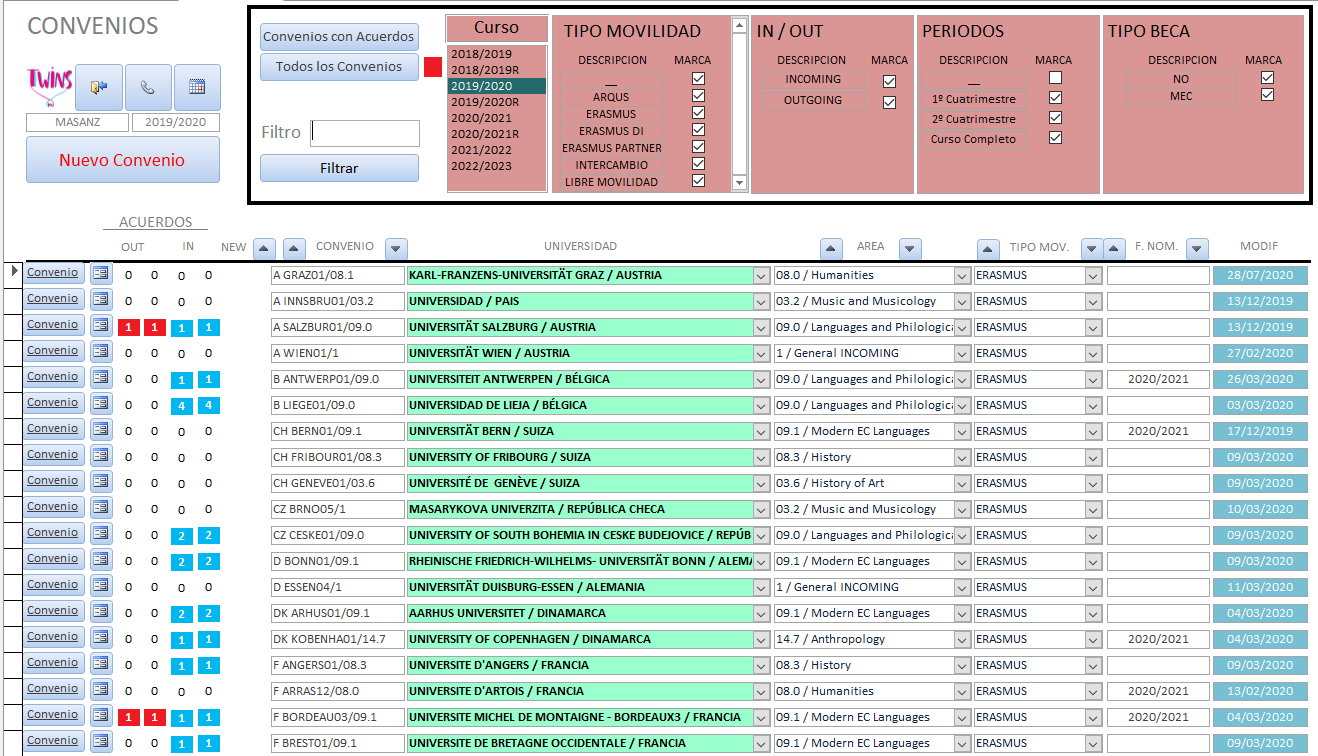
\includegraphics[width=\textwidth]{img/Capturas de TWINS/vistaConvenios.png}
	\caption{Vista de Convenios}
	\label{vistaConvenios}
\end{figure}

\begin{table}[h]
	\begin{center}
		\begin{tabular}{ | c | c | } 
			\hline
			\multicolumn{2}{|c|}{\textbf{Administración}} \\
			\hline
			Estudiantes \footnotemark & 2055 \\ 
			\hline
			Tutores & 58 \\
			\hline
			Convenios  & 607 \\ 
			\hline
			Expedientes & 5049 \\ 
			\hline
			\multicolumn{2}{|c|}{\textbf{Base de datos}} \\
			\hline
			Tablas & 108 \\
			\hline
			Relaciones & 60 \\
			\hline
			Macros & 55 \\
			\hline
			Formularios & 152 \\
			\hline
		\end{tabular}
		\caption{Estadísticas de TWINS}
		\label{estadisticasTWINS}
	\end{center}
\end{table}~
\footnotetext{Tanto \textit{incoming} como \textit{outcoming}}



\subsubsection{El modelo de datos}

El modelo entidad-relación es el elegido para el diseño de esta base de datos. Las distintas tablas de la misma se conectan mediante relaciones que establecen restricciones para mantener la consistencia entre los datos.

Las relaciones pueden ser:
\begin{itemize}
	\item \textbf{Uno-a-uno}
\end{itemize}
